\documentclass{beamer}
\usepackage[utf8]{inputenc}

\usepackage{amsmath,amsfonts,amssymb,amsthm,
mathtools,mathrsfs}
\usepackage{physics}
\usepackage{xcolor}
\usepackage{listings}
\usepackage{caption, subcaption}
\usepackage{pgf-pie}
\usepackage{hyperref}

\usetheme{Madrid}
\usecolortheme{default}
\useoutertheme[subsection=false]{miniframes}

\addtobeamertemplate{block example begin}{%
    \setlength{\textwidth}{0.8\textwidth}
}{}

\usepackage[style=apa, backend=biber, natbib]{biblatex}
\addbibresource{references.bib}


\title[LSD Analysis]{Liquidity Unleashed: A Research-driven Analysis of Post-Shanghai LSDs}
\subtitle{Science of Blockchain Conference - DFS Forum}
\author[Mingxuan He]{
    Mingxuan He\\ 
    mingxuanh.eth
    }


\institute[]{
Phoenix graduate scholar (computational economics), University of Chicago\\
Research fellow, Nethermind
}


\date{\today}


% table of contents page before each section (optional)
% \AtBeginSection[]
% {
%   \begin{frame}
%     \frametitle{Table of Contents}
%     \tableofcontents[currentsection]
%   \end{frame}
% }


\begin{document}

% title page
\begin{frame}
\titlepage  
\end{frame}

% table of contents
\begin{frame}
\frametitle{Table of Contents}
\tableofcontents
\end{frame}


%----------------
\section[Introduction]{Introduction to Ethereum Staking \& LSDs}
\begin{frame}{History of Ethereum Staking}

    \begin{itemize}
        \item The Merge (Sep 2022): Ethereum migrated from PoW to PoS\\
        $\Rightarrow$ Now anyone can stake $32\Xi$ on mainnet and accrue rewards as a validator
        \bigskip
        \item The Shanghai/Capella Upgrade (Apr 2023) \\
        $\Rightarrow$ Introduced option to withdraw staked ETH (unstake)
    \end{itemize}

    
\end{frame}

\begin{frame}{Breakdown of Ethereum Staking Rewards}
\begin{itemize}
    \item Consensus layer rewards: Attestation, block proposal, sync committee
    \item Execution layer rewards: Txn fee (EIP-1559), MEV
\end{itemize}
\begin{figure}
    \centering
    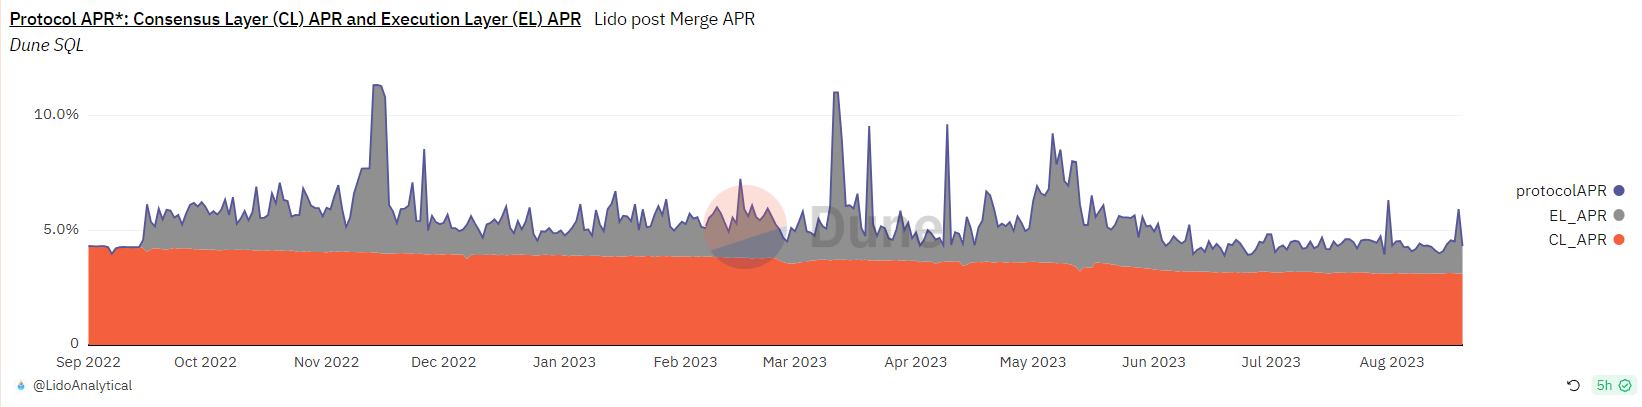
\includegraphics[width=\textwidth]{figures/lido_apr.png}
\end{figure}
\tiny{source: \href{https://dune.com/LidoAnalytical/lido-execution-layer-rewards}{@LidoAnalytical on Dune}}

\end{frame}



\begin{frame}{ETH Staking Landscape}
    \begin{figure}
        \centering
        \begin{subfigure}[b]{0.45\textwidth}
            \centering
            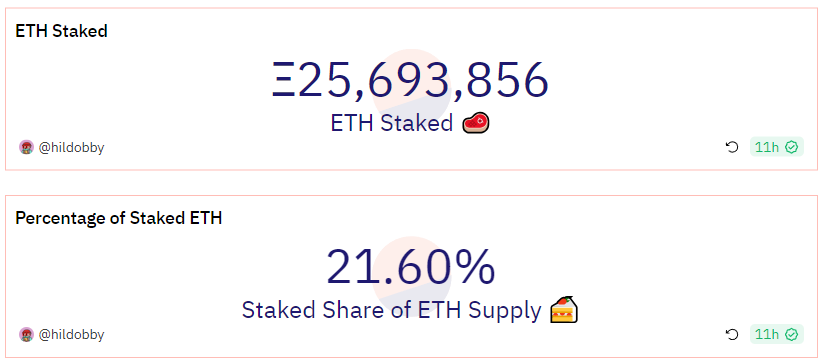
\includegraphics[width=\textwidth]{figures/eth_stake_stats.png}
        \end{subfigure}
        \begin{subfigure}[b]{0.45\textwidth}
            \centering
            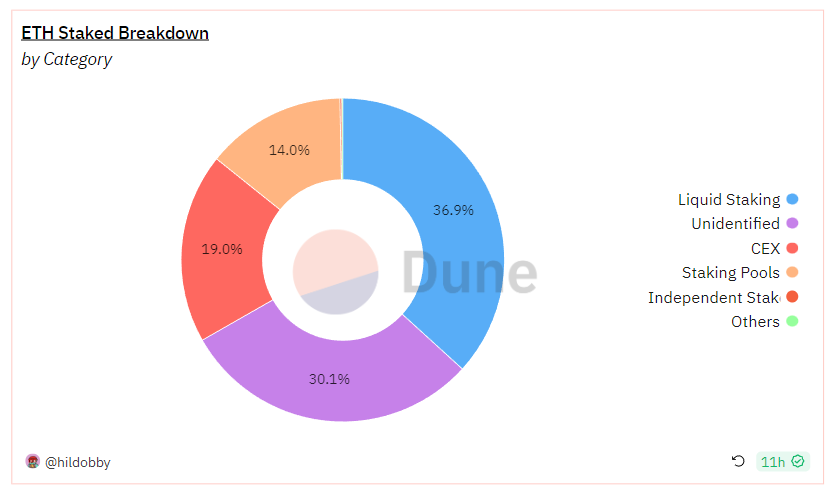
\includegraphics[width=\textwidth]{figures/eth_stake_breakdown.png}
        \end{subfigure}
    \end{figure}
    \tiny{source: \href{https://dune.com/hildobby/eth2-staking}{@hildobby on Dune}}

\end{frame}

\begin{frame}{Liquid Staking Derivatives (LSDs)}
    ERC-20 tokens that represent ETH tokens locked in PoS contracts. 
    \begin{itemize}
        \item Benefits of LSD: yields staking rewards \& has liquidity
        \item Liquid use cases: borrowing/lending, trading portfolio collateral, etc.
        \item LSDs are redeemable for ETH at any time
        \item Most LSDs accrue rewards automatically i.e. \textbf{holding LSDs is equivalent to staking ETH in the pool}
    \end{itemize}
    \bigskip
    
\end{frame}

\begin{frame}{LSDs saw huge growth after Shapella}
    \begin{figure}
        \centering
        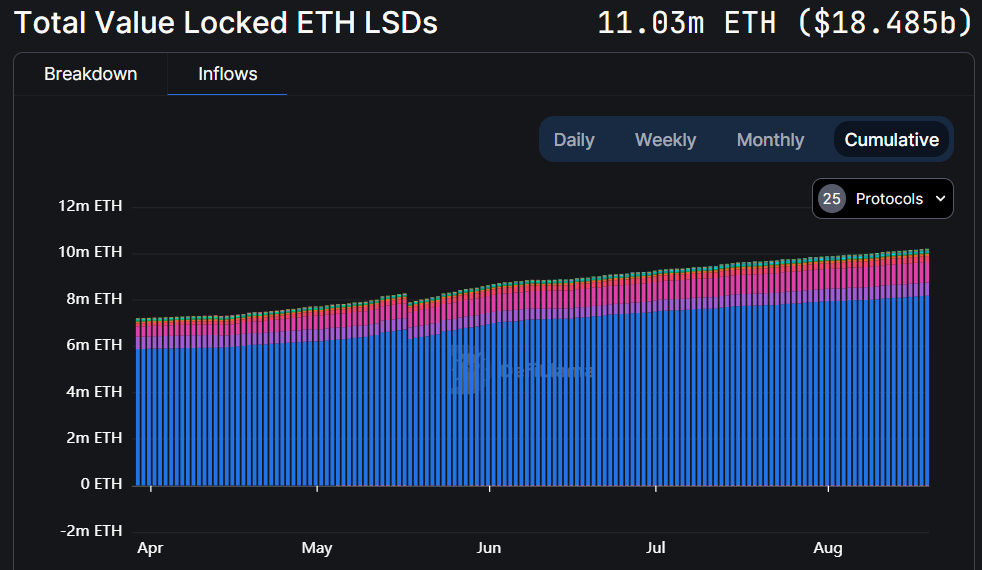
\includegraphics[width=0.8\textwidth]{figures/lsd_2023.png}
    \end{figure}
    \tiny{source: \href{https://defillama.com/lsd}{DeFi Llama}}
    
\end{frame}

%----------------
\section[Economic Analysis]{Economic \& Financial Risk Analysis of LSDs}
\begin{frame}{Liquid Staking Protocols as Banks}

    \footnotemark Banks are financial intermediaries which create liquidity by:

    \begin{itemize}
        \item Gathering liquid funds (e.g. customer deposits) as liabilities
        \item Holding illiquid investment projects (e.g. loans, bonds) as assets
    \end{itemize}
    \bigskip
    Similarly, LSD protocols create liquidity by:
    \begin{itemize}
        \item Gathering liquid funds (ETH) as liabilities
        \item Holding in illiquid investment projects (Ethereum staking) as assets
    \end{itemize}

    % % use columns
    % \begin{tabular}{|c|c|c|}
    %     \hline
    %      & Banks & Liquid Staking Pools \\
    %     \hline
    %     Invests in & Loans & ETH validators \\
    %     \hline
    %     Deposits & Checking accounts & ETH deposits \\
    %     \hline
    % \end{tabular}

\footnotetext{Diamond and Dybvig (1983) Theory of Banking}
\end{frame}

% \begin{frame}{Supply and Demand Analysis}
    
% \end{frame}

\begin{frame}{How Much Liquidity do LSDs Provide?}
    Introducing two quantitative measures of (il)liquidity:\\
    \textcircled{1} Amihud (2002):
    $AMD_{id} = \frac{1}{N_id}\sum_{t=1}^{N_{id}}\frac{|r_{it}|}{V_t}$
    \begin{figure}
        \centering
        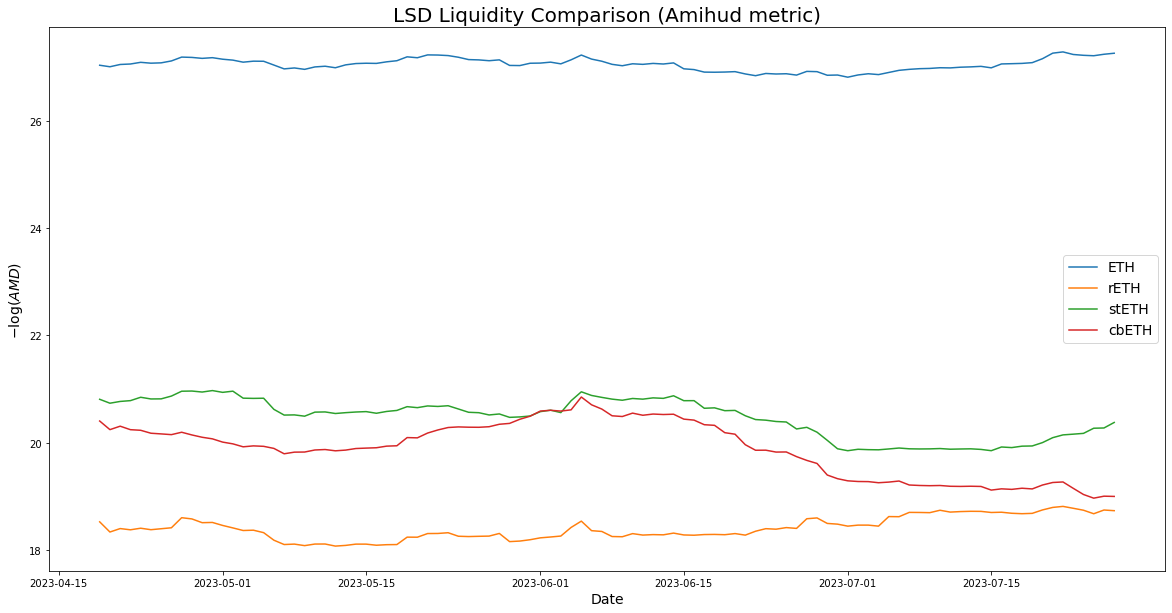
\includegraphics[width=\textwidth]{figures/liq_AMD.png}
    \end{figure}
\end{frame}

\begin{frame}
    \textcircled{2} Bao, Pan, and Wang (2011): $\gamma_i = -Cov(\Delta p_{it}, \Delta p_{it-1})$
    \begin{figure}
        \centering
        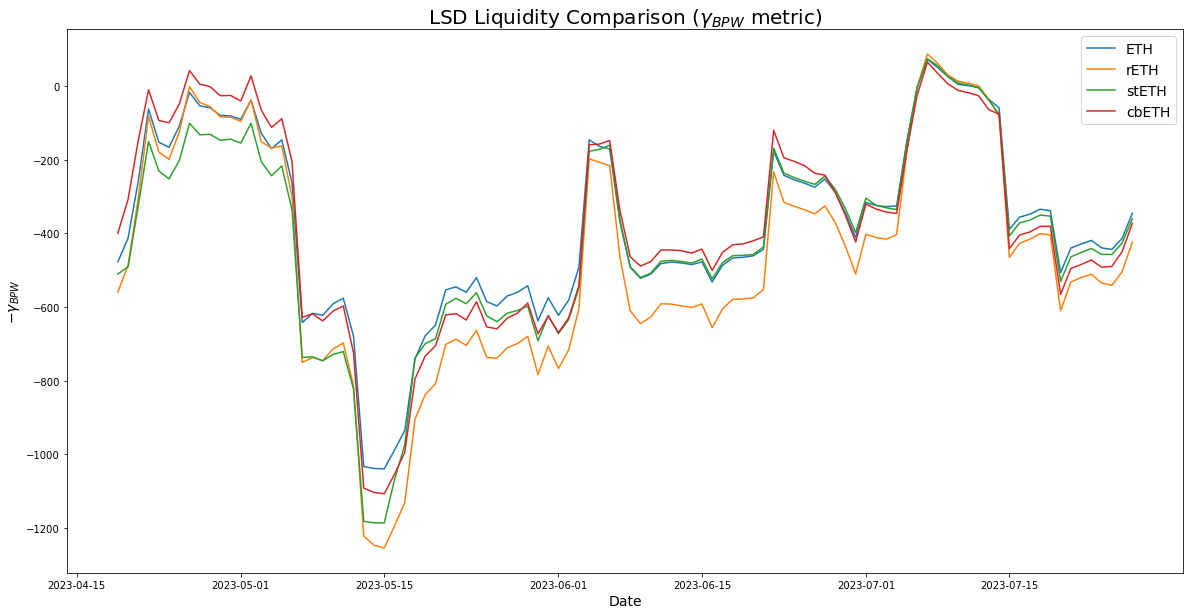
\includegraphics[width=\textwidth]{figures/liq_BPW.png}
    \end{figure}
\end{frame}

\begin{frame}{Are LSD Bank Runs Possible?}
    Bank runs are typically triggered by 1. sudden increase in demand for liquidity 2. expectation of protocol insolvency.\\  
    \bigskip
    \begin{itemize}
        \item Liquidity shortage: e.g. CRV exploit July 2023 where multiple liquidity pools were drained
        \item ETH price drop
        \item Regulatory crackdown: e.g. SEC deems LSDs as securities
        \item Large-scale slashing or penalty of validators
        \item Bugs/exploits/hacks stealing protocol funds
    \end{itemize}
\end{frame}


\begin{frame}{During a LSD Bank Run:}
    Two main methods of converting LSDs back to ETH:
    \begin{itemize}
        \item Direct redemption from protocol (deposit pool / POL)
        \item Through DEX pools/aggregators
    \end{itemize}
    \bigskip
    What happens after these run out?\\
\end{frame}

\begin{frame}{Withdrawing Staked ETH from Validators}
    \begin{itemize}
        \item Step 1: Exit queue -- only 10 validators can exit per epoch ($\approx$2225 validators or 0.5\% circulating supply per day).
        \item Step 2: Withdrawl queue -- same queue with partial withdrawls but is processed much slower
    \end{itemize}
    \begin{figure}
        \centering
        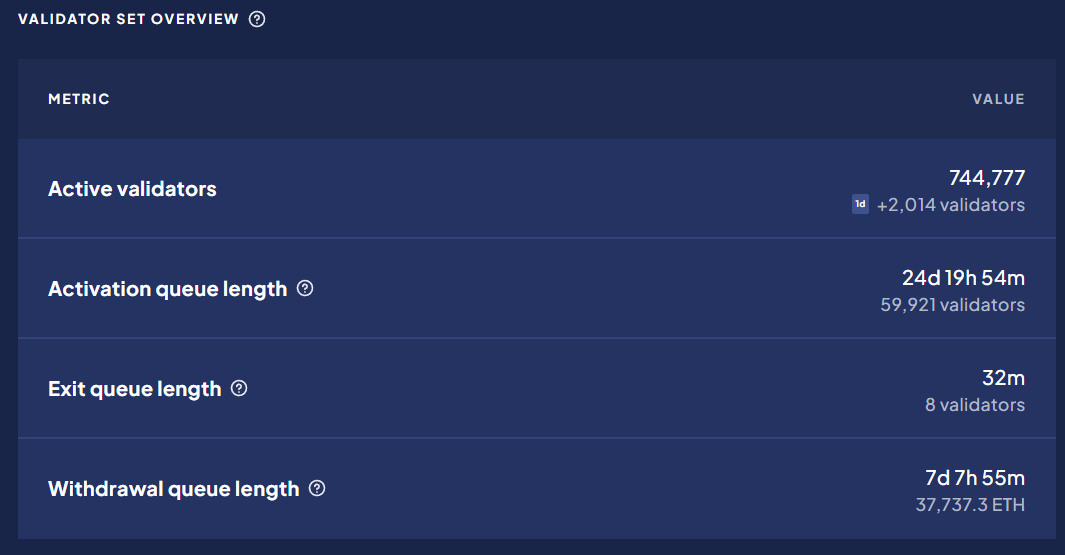
\includegraphics[width=0.8\textwidth]{figures/rated_queues.png}
    \end{figure}
    \tiny{source: \href{https://www.rated.network/overview?network=mainnet&timeWindow=30d&rewardsMetric=average}{Rated Network}}\\
    https://notes.ethereum.org/@launchpad/withdrawals-faq
\end{frame}

\begin{frame}{Last resort}
    \begin{itemize}
        \item Pause/delay withdrawals (e.g. Lido's Bunker Mode)
        \item Sell protocol assets (e.g. gov tokens) !!Might cause self-fulfilling prophecy of insolvency!!
    \end{itemize}
    
\end{frame}

\begin{frame}{Systemic Risks}
    \begin{itemize}
        \item Centralization of stake (esp. Lido): Nethermind Research and Lido are collaborating to solve this\footnotemark! Also DVT
        \item APR drop from excessive staking (block rewards do not scale linearly with ETH staked)
        \item ETH supply inflation if staking $>>$ usage (ETH minted $>>$ burned by EIP-1559)
    \end{itemize}

    \footnotetext{See \href{https://medium.com/nethermind-eth/a-path-to-permissionless-liquid-staking-9934557f6d20}{``A Path to Permissionless Liquid Staking"} by Nethermind \& LidoDAO}
\end{frame}

%----------------
\section[Rocket Pool Case Study]{Rocket Pool Case Study}

\begin{frame}{Rocket Pool (rETH)}
    \begin{figure}
        \centering
        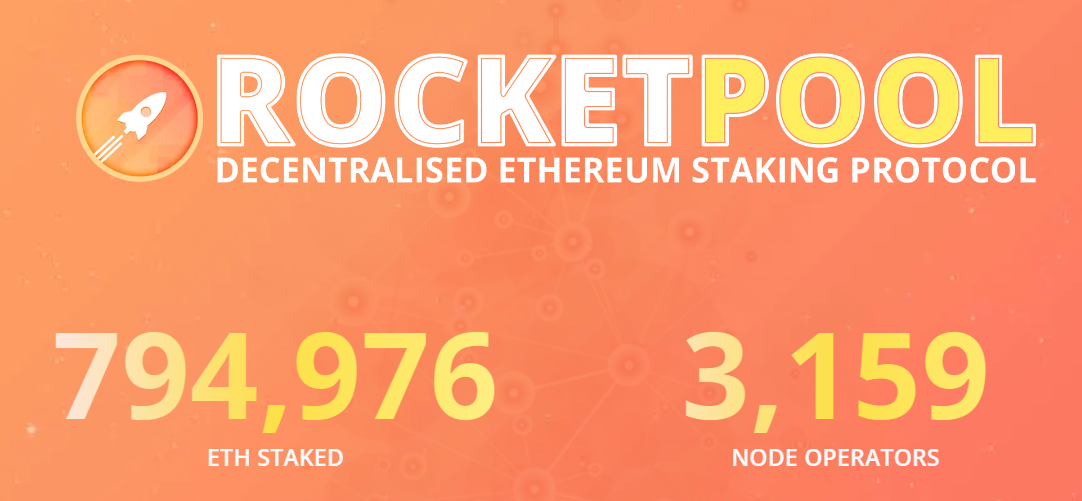
\includegraphics[width=0.8\textwidth]{figures/rpl_logo.png}
    \end{figure}
    Rocket Pool is the 3rd largest LSD protocol by TVL and the largest \textbf{permissionless} LSD protocol.
\end{frame}

\begin{frame}{rETH Liquidity Analysis}
    (Data as of Aug 26, 2023)
    \begin{align*}
        &\text{Balancer v2 rETH-WETH pool} & 12,893\Xi\\
        &\text{Balancer v2 rETH-wstETH-sfrxETH pool} & 11,307\Xi\\
        &\text{Curve v2 rETH-ETH pool} & 2,238\Xi\\
        &\text{Uniswap v3 rETH-ETH pool} & 1,007\Xi\\
        \hline
        &\text{Total DEX Liquidity} & 27,445\Xi\\
        &\text{Protocol Owned Liquidity (Deposit Pool)} & 18,000\Xi\\
        \hline
        &\text{Total Liquidity} & 45,445\Xi\\
    \end{align*}
    This is only 5\% of rETH supply (902,768$\Xi$), or 4\% if not counting other LSDs as liquidity.
\end{frame}

\begin{frame}{Rocket Pool Agent-Based Model \& Simulation}
    I've been building an agent-based simulation model for Rocket Pool to study and improve their protocol design. Areas I focused on include:\\
    \begin{itemize}
        \item rETH and RPL tokenomics
        \item Behavior of node operators
        \item Response to external risks
    \end{itemize}
\end{frame}

\begin{frame}
    \begin{figure}
        \centering
        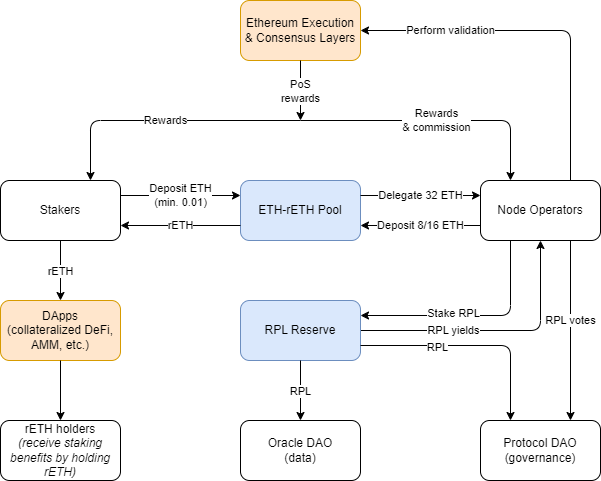
\includegraphics[width=0.8\textwidth]{figures/Rocketpool tokenomics.png}
    \end{figure}
\end{frame}

\begin{frame}{Thank You!}
    Connect with me on Twitter/Telegram @MingXDynasty, and Linkedin!\\ 
    \bigskip
    \begin{itemize}
        \item Check out \href{https://www.mingxuanhe.xyz/}{\underline{mingxuanhe.xyz}} for more research in DeFi \& cryptoeconomics
        % \item Support my community-funded 
        % \href{https://explorer.gitcoin.co/\#/round/10/0xc5fdf5cff79e92fac1d6efa725c319248d279200/0xc5fdf5cff79e92fac1d6efa725c319248d279200-0}{\underline{research grant on Gitcoin}}
        \item I'm on the job market for 2024!
 
    \end{itemize}
   

\end{frame}

\section*{}

\begin{frame}[allowframebreaks]{References}
    \nocite{*}
    \printbibliography
\end{frame}


\end{document}
